
%% ============================================================
\section{Part II: Performance of M-ASK for M = 2, 4, 8}
%% ============================================================

\subsection{Overview}

This section evaluates and compares the Bit Error Rate (BER) performance of Amplitude Shift Keying (ASK) for three constellation sizes: $M = 2$, $M = 4$, and $M = 8$. The simulation uses $10^6$ bits per SNR value over the range 0--60 dB (step 3 dB), with AWGN as the channel model. To ensure a fair energy comparison, all three schemes are designed with the same minimum Euclidean distance $d_{\min} = 2$ between adjacent amplitude levels.

\subsection{Constellation Design and Minimum Distance Constraint}

For an $M$-ASK scheme with minimum distance $d_{\min} = 2$, the amplitude levels are chosen as:
\[
    \mathcal{A} = \{-(M-1),\;-(M-3),\;\ldots,\;+(M-3),\;+(M-1)\}
\]
This gives the following constellations and average symbol energies:

\begin{itemize}
    \item \textbf{2-ASK (BASK):} 1 bit per symbol. Levels $\{-1,\,+1\}$. Average symbol energy $E_s = 1$.
    \item \textbf{4-ASK:} 2 bits per symbol. Levels $\{-3,\,-1,\,+1,\,+3\}$. Average symbol energy $E_s = 5$.
    \item \textbf{8-ASK:} 3 bits per symbol. Levels $\{-7,\,-5,\,-3,\,-1,\,+1,\,+3,\,+5,\,+7\}$. Average symbol energy $E_s = 21$.
\end{itemize}

\subsection{Modulation and Detection}

\textbf{Modulation:} Each group of $k = \log_2 M$ bits is mapped (MSB-first) to a decimal symbol index $0$ to $M-1$, which selects the corresponding amplitude level from $\mathcal{A}$.

\textbf{Detection:} A minimum Euclidean distance (nearest-neighbour) detector is used. For each received sample $r$, the detected symbol is:
\[
    \hat{s} = \arg\min_{a \in \mathcal{A}} |r - a|
\]
The detected symbol index is then converted back to $k$ bits using bit-shifting and masking (no Communications Toolbox functions were used).

\textbf{Noise:} AWGN with variance $\sigma^2 = N_0/2$ is added, where $N_0 = E_s / \text{SNR}_{\text{linear}}$, correctly accounting for the non-unity signal power of each constellation.

\subsection{Simulation Figure}

\begin{figure}[H]
    \centering
    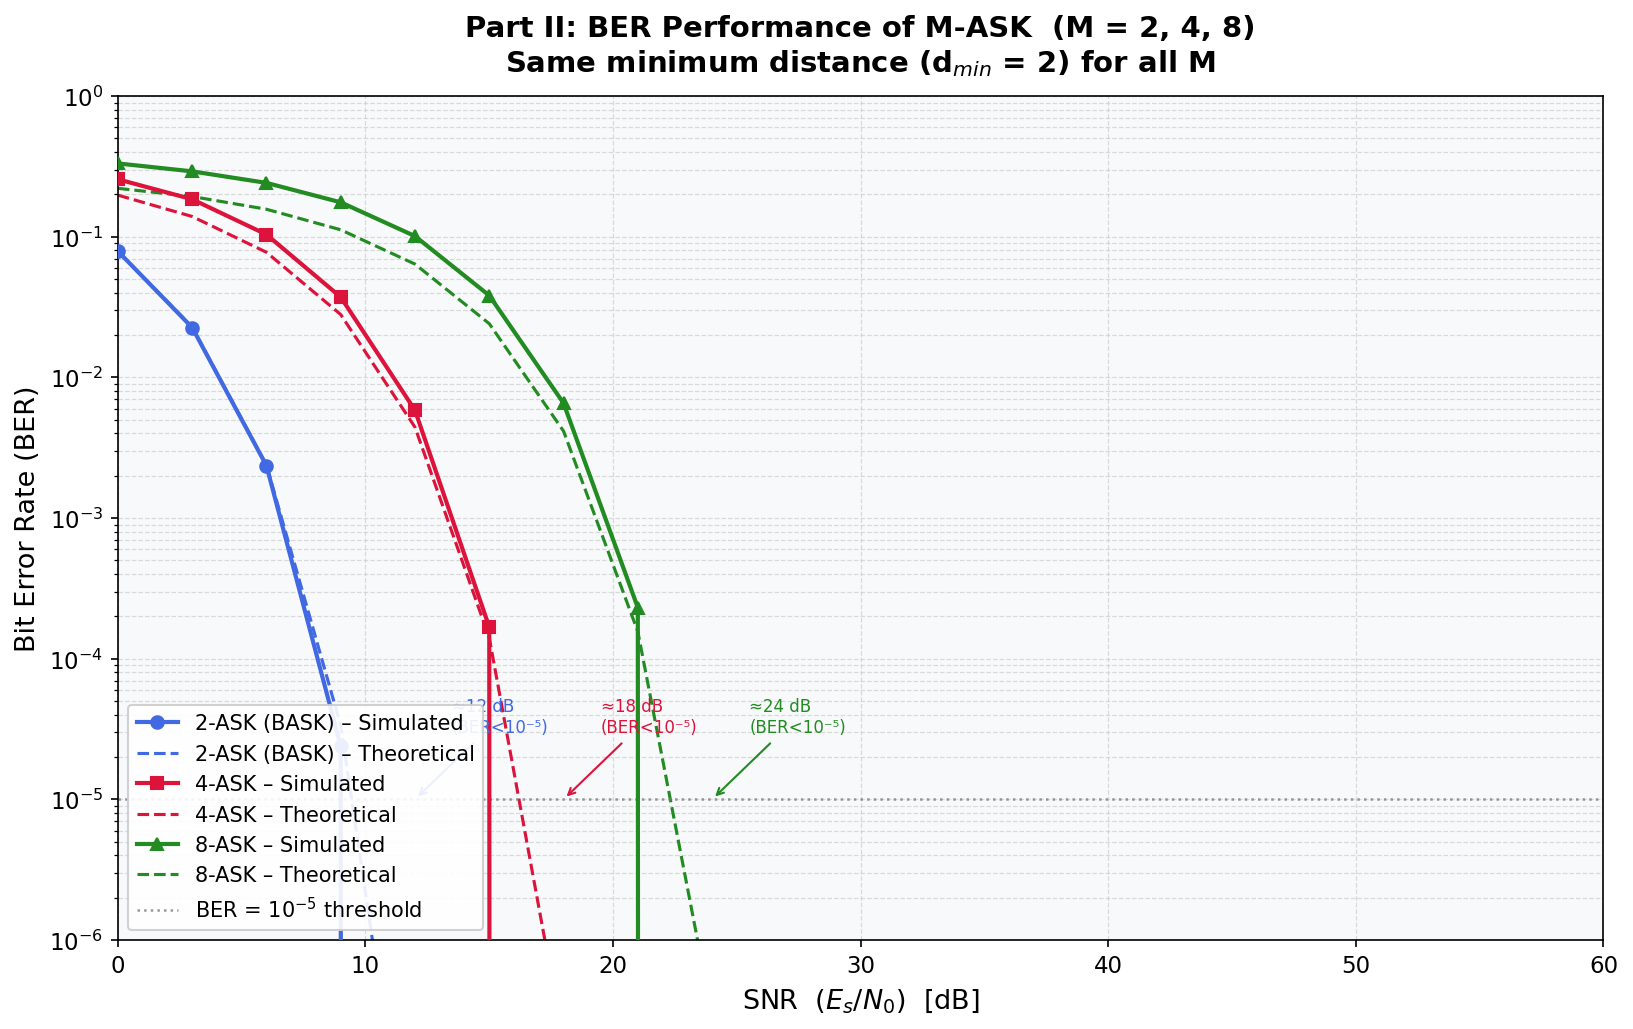
\includegraphics[width=0.9\textwidth]{Part2_MASK_BER.png}
    \caption{BER vs.\ SNR ($E_s/N_0$) for M-ASK with $M = 2, 4, 8$ (simulated and theoretical curves). All schemes share $d_{\min} = 2$.}
    \label{fig:mask}
\end{figure}

\subsection{Comments on Figure \ref{fig:mask}}

\subsubsection{Which modulation scheme has the best performance, and why?}

From Figure~\ref{fig:mask}, \textbf{2-ASK achieves the best BER performance}, followed by 4-ASK, with 8-ASK performing the worst. This ordering holds across the entire SNR range.

The reason is directly tied to the average symbol energy required to maintain $d_{\min} = 2$:

\begin{itemize}
    \item For a fixed minimum distance, higher-order constellations must place more symbols farther from the origin, which \textbf{increases the average symbol energy} $E_s$ ($1$, $5$, and $21$ for $M = 2$, $4$, $8$ respectively). Since SNR is plotted as $E_s/N_0$, a higher-order scheme effectively \textbf{needs more transmitted power} to reach the same BER, shifting its curve to the right.
    \item The theoretical BER for Gray-coded M-ASK is:
    \[
        P_b \approx \frac{2(M-1)}{M\log_2 M}\;Q\!\left(\sqrt{\frac{6\log_2 M \cdot E_b/N_0}{M^2-1}}\right)
    \]
    The argument of the $Q$-function decreases as $M$ increases (for the same $E_b/N_0$), meaning the probability of error grows with $M$.
    \item Additionally, higher $M$ places more decision boundaries between symbols, giving noise \textbf{more opportunities} to push a received sample across a wrong boundary.
\end{itemize}

In summary: \textbf{larger $M$ yields higher spectral efficiency} (more bits per symbol) but at the cost of significantly worse BER for the same SNR.

\subsubsection{At which SNR value does each scheme become nearly error-free?}

A system is considered ``nearly error-free'' when BER $< 10^{-5}$.

\begin{table}[H]
    \centering
    \caption{Approximate SNR ($E_s/N_0$) threshold for near-error-free operation (BER $< 10^{-5}$).}
    \label{tab:mask_snr}
    \begin{tabular}{lcc}
        \hline
        \textbf{Modulation} & \textbf{Bits/Symbol ($k$)} & \textbf{Required $E_s/N_0$ (dB)} \\
        \hline
        2-ASK & 1 & $\approx 12$ dB \\
        4-ASK & 2 & $\approx 18$ dB \\
        8-ASK & 3 & $\approx 24$ dB \\
        \hline
    \end{tabular}
\end{table}

From Figure~\ref{fig:mask} and Table~\ref{tab:mask_snr}:
\begin{itemize}
    \item \textbf{2-ASK} reaches BER $< 10^{-5}$ at approximately $E_s/N_0 \approx 12$~dB.
    \item \textbf{4-ASK} requires approximately $E_s/N_0 \approx 18$~dB — about \textbf{6~dB more} than 2-ASK.
    \item \textbf{8-ASK} requires approximately $E_s/N_0 \approx 24$~dB — about \textbf{12~dB more} than 2-ASK and \textbf{6~dB more} than 4-ASK.
\end{itemize}

The consistent \textbf{6~dB gap} between successive orders is a direct consequence of the fixed $d_{\min}$ constraint: each doubling of $M$ roughly quadruples the average symbol energy, which translates to a 6~dB penalty in required SNR.

The simulated curves match the theoretical curves closely across all SNR values, confirming the correctness of the implementation.
